\documentclass[crop,tikz]{standalone}
\begin{document}
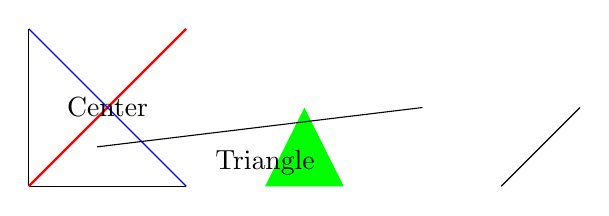
\begin{tikzpicture}
  % Basic lines
  \draw (0,0) -- (2,0);
  \draw (0,0) -- (0,2);

  % Colored and styled lines
  \draw[red,thick] (0,0) -- (2,2);
  \draw[blue] (2,0) -- (0,2);

  % Filled shapes
  \fill[green] (3,0) -- (4,0) -- (3.5,1) -- cycle;

  % Polar coordinates
  \draw (5,1) -- (30:1);

  % Nodes
  \node at (1,1) {Center};
  \node at (3,0.3) {Triangle};

  % Named coordinates
  \coordinate (A) at (6,0);
  \coordinate (B) at (7,1);
  \draw (A) -- (B);
\end{tikzpicture}
\end{document}
